\documentclass{article}

\usepackage[top=1.5cm,bottom=0.5cm,left=0.5cm,right=0.5cm]{geometry}
\usepackage{xeCJK}
\usepackage{fontspec}
\usepackage{listings}
\usepackage{fancyhdr}
\usepackage{changepage}
\usepackage{color}
\usepackage{amsmath}
\usepackage{amssymb}
\usepackage{amsthm}
\usepackage{graphicx}
\usepackage{tikz}
\usepackage{algpseudocode}
\setCJKmainfont{Noto Serif CJK TC}
\setmonofont{Consolas}

\lstset{
language=C++,
basicstyle=\ttfamily\footnotesize,
tabsize=2,
breaklines=true,
breakatwhitespace=false,
escapeinside={\%*}{*)},
morekeywords={*}
}

\newcommand{\makegrid}{
\clearpage

\begin{center}
    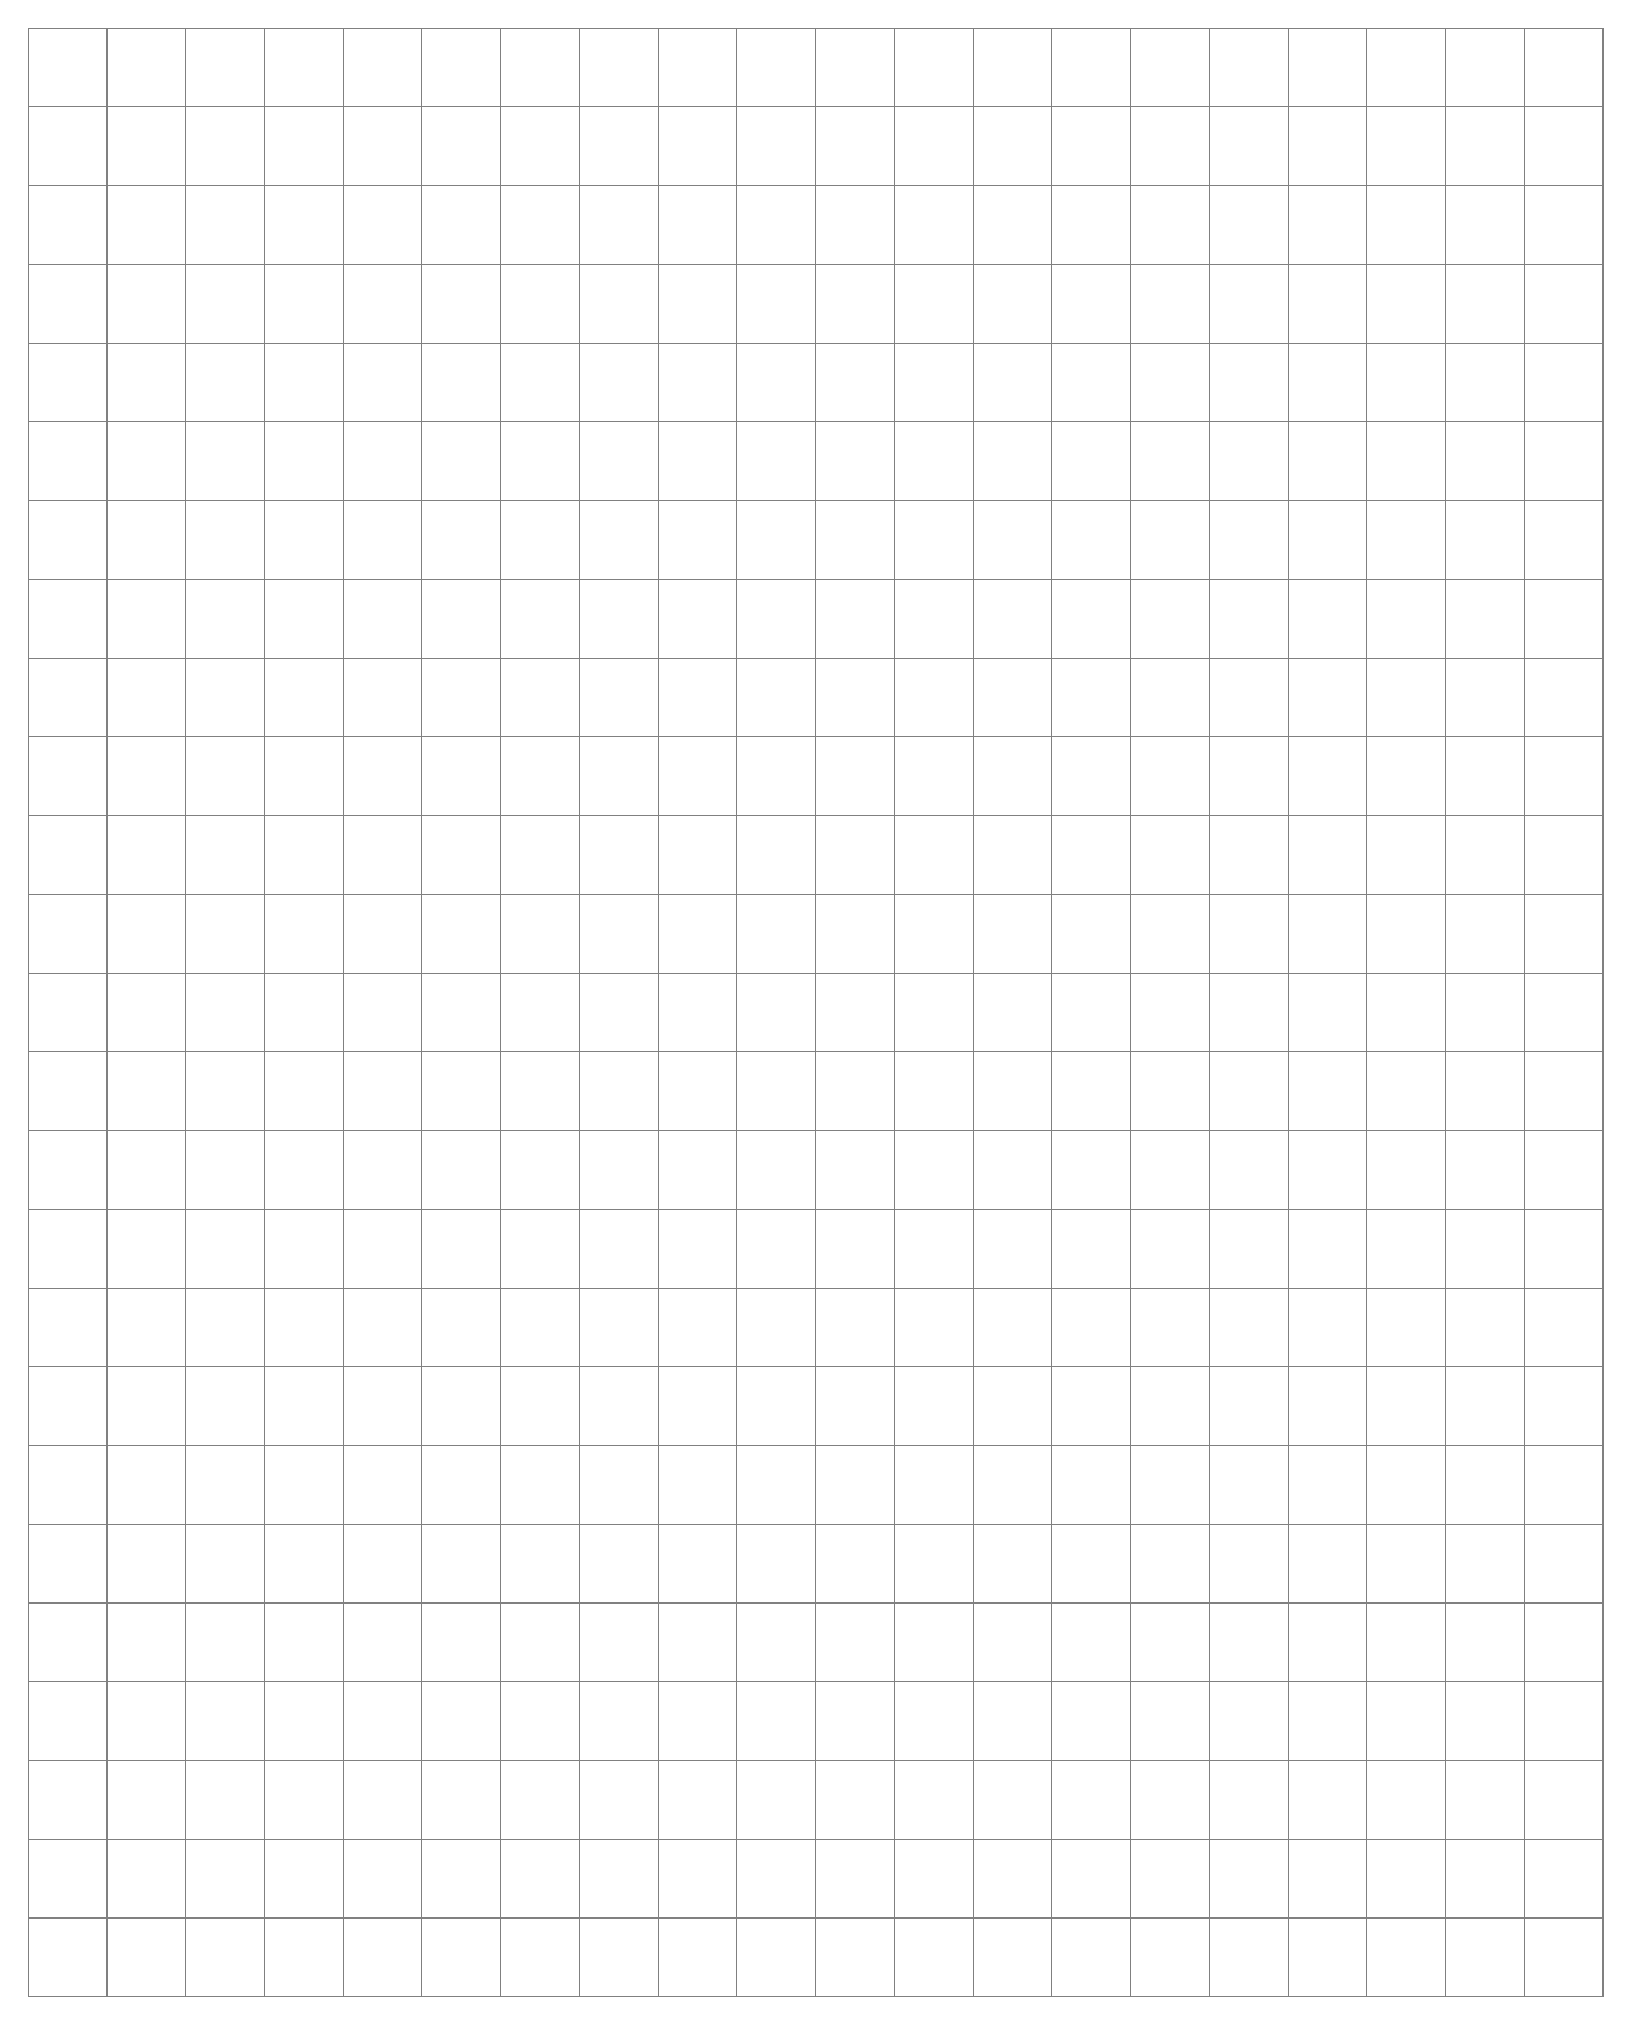
\begin{tikzpicture}
        \draw[step=1, gray, thin] (0,0) grid (20.0, 25.0);
    \end{tikzpicture}
\end{center}
}

\begin{document}

\setlength\parindent{0pt}
\setlength\columnseprule{0.5pt}
\footnotesize


\pagestyle{fancy}
\fancyfoot{}
\fancyhead[L]{National Taiwan University}
\fancyhead[C]{ideograph\_advantage}
\fancyhead[R]{\thepage}

\twocolumn

\tableofcontents

\section{Basic}

\subsection{Default Code}
\lstinputlisting{Basic/template.cpp}

\subsection{.vimrc}
\lstinputlisting{Basic/vimrc}

\subsection{Fast IO}
\lstinputlisting{Basic/fastio.cpp}

\subsection{Random}
\lstinputlisting{Basic/random.cpp}

\subsection{Checker}
\lstinputlisting{Basic/checker.sh}

\section{Data Structure}

\subsection{Heavy-Light Decomposition}
\lstinputlisting{DataStructure/HLD.cpp}

%\subsection{Li-Chao Tree}
%\lstinputlisting{DataStructure/LiChao.cpp}

\subsection{Link Cut Tree}
\lstinputlisting{DataStructure/LinkCutTree.cpp}

\subsection{Treap}
\lstinputlisting{DataStructure/treap.cpp}

\section{Flow Matching}


\subsection{Dinic}
\lstinputlisting{Flow_Matching/Dinic.cpp}

\subsection{Bounded Flow}
\lstinputlisting{Flow_Matching/Bounded_flow.cpp}

\subsection{Gomory Hu}
\lstinputlisting{Flow_Matching/GomoryHu.cpp}

\subsection{Hungarian Algorithm}
\lstinputlisting{Flow_Matching/Hungarian.cpp}

\subsection{ISAP Algorithm}
\lstinputlisting{Flow_Matching/isap.cpp}

\subsection{Bipartite Matching}
\lstinputlisting{Flow_Matching/BipartiteMatching.cpp}

\subsection{Max Simple Graph Matching}
\lstinputlisting{Flow_Matching/Max_Simple_Graph_Matching.cpp}

\subsection{MCMF}
\lstinputlisting{Flow_Matching/MCMF.cpp}

\subsection{Min Cost Circulation}
\lstinputlisting{Flow_Matching/MinCostCirculation.cpp}

\subsection{SW Mincut}
\lstinputlisting{Flow_Matching/SW_mincut.cpp}

\section{Geometry}

\subsection{Geometry Template}
\lstinputlisting{Geometry/GeometryTemplate.cpp}

\subsection{Convex Hull}
\lstinputlisting{Geometry/ConvexHull.cpp}

\subsection{Minimum Enclosing Circle}
\lstinputlisting{Geometry/MinimumEnclosingCircle.cpp}

\subsection{Minkowski Sum}
\lstinputlisting{Geometry/MinkowskiSum.cpp}

\subsection{Polar Angle Comparator}
\lstinputlisting{Geometry/PolarAngleComp.cpp}

\subsection{Half Plane Intersection}
\lstinputlisting{Geometry/HalfPlaneIntersection.cpp}

\subsection{Dynamic Convex Hull}
\lstinputlisting{Geometry/DynamicConvexHull.cpp}

\subsection{3D Point}
\lstinputlisting{Geometry/3DPoint.cpp}

\subsection{ConvexHull3D}
\lstinputlisting{Geometry/ConvexHull3D.cpp}

\subsection{Circle Operations}
\lstinputlisting{Geometry/CircleOperations.cpp}

\subsection{Delaunay Triangulation}
\lstinputlisting{Geometry/DelaunayTriangulation.cpp}

\subsection{Voronoi Diagram}
\lstinputlisting{Geometry/VoronoiDiagram.cpp}

\section{Graph}

\subsection{Block Cut Tree}
\lstinputlisting{Graph/BlockCutTree.cpp}

\subsection{2-SAT}
\lstinputlisting{Graph/2SAT.cpp}

\subsection{Dominator Tree}
\lstinputlisting{Graph/DominatorTree.cpp}

\subsection{Virtual Tree}
\lstinputlisting{Graph/VirtualTree.cpp}

\subsection{Directed Minimum Spanning Tree}
\lstinputlisting{Graph/DirectedMST.cpp}

\subsection{Vizing}
\lstinputlisting{Graph/Vizing.cpp}

\subsection{Maximum Clique}
\lstinputlisting{Graph/MaximumClique.cpp}

\section{Math}

\subsection{Extended Euclidean Algorithm}
\lstinputlisting{Math/ExtGCD.cpp}

\subsection{Floor \& Ceil}
\lstinputlisting{Math/floor_ceil.cpp}

\subsection{Legendre}
\lstinputlisting{Math/Legendre.cpp}

\subsection{Simplex}
\lstinputlisting{Math/Simplex.cpp}

\subsection{Floor Sum}
\lstinputlisting{Math/FloorSum.cpp}

\subsection{DiscreteLog}
\lstinputlisting{Math/DiscreteLog.cpp}

\subsection{Miller Rabin \& Pollard Rho}
\lstinputlisting{Math/MillerRabin_PollardRho.cpp}

\subsection{XOR Basis}
\lstinputlisting{Math/Basis.cpp}

\subsection{Linear Equation}
\lstinputlisting{Math/LinearEquation.cpp}

\section{Misc}

\subsection{Fraction}
\lstinputlisting{Misc/Fraction.cpp}

\subsection{Matroid}
% From IOIC 2021,2022
我們稱一個二元組 $M = (E, \mathcal{I})$ 為一個擬陣,
其中 $\mathcal{I} \subseteq 2^E$ 為 $E$ 的子集所形成的\textbf{非空}集合,若:

\begin{itemize}
    \item 若 $S \in \mathcal{I}$ 以及 $S^\prime \subsetneq S$,則
        $S^\prime \in \mathcal{I}$
    \item 對於 $S_1, S_2 \in \mathcal{I}$ 滿足 $|S_1| < |S_2|$,存在
        $e \in S_2 \setminus S_1$ 使得 $S_1 \cup \{e\} \in \mathcal{I}$
\end{itemize}

除此之外,我們有以下的定義:

\begin{itemize}
    \item 位於 $\mathcal{I}$ 中的集合我們稱之為獨立集(independent set),反之不在
        $\mathcal{I}$ 中的我們稱為相依集(dependent set)
    \item 極大的獨立集為基底(base)、極小的相依集為迴路(circuit)
    \item 一個集合 $Y$ 的秩(rank)$r(Y)$ 為該集合中最大的獨立子集,也就是
        $r(Y) = \max\{|X| \mid X \subseteq Y \text{ 且 } X \in \mathcal{I} \}$
\end{itemize}

性質:
\begin{enumerate}
    \item $X \subseteq Y \land Y \in \mathcal I \implies X \in \mathcal I$
    \item $X \subseteq Y \land X \notin \mathcal I \implies Y \notin \mathcal I$
    \item 若 $B$ 與 $B'$ 皆是基底且 $B \subseteq B'$,則 $B=B'$\\
          若 $C$ 與 $C'$ 皆是迴路且 $C \subseteq C'$,則 $C=C'$
    \item $e \in E \land X \subseteq E \implies r(X) \leq r(X \cup \{e\}) \leq r(X) + 1$ i.e. 加入一個元素後秩不會降底,最多增加 1
    \item $\forall Y \subseteq E, \exists X \subseteq Y, r(X)=\lvert X \rvert = r(Y)$
\end{enumerate}

一些等價的性質:
\begin{enumerate}
    \item 對於所有 $X \subseteq E$,$X$ 的極大獨立子集都有相同的大小
    \item 對於 $B_1,B_2 \in \mathcal B \land B_1 \neq B_2$,
        對於所有 $e_1 \in B_1 \setminus B_2$,
        存在 $e_2 \in B_2 \setminus B_1$ 使得 $(B_1 \setminus \{e_1\}) \cup \{e_2\} \in \mathcal B$
    \item 對於 $X,Y \in \mathcal I$ 且 $\lvert X \rvert < \lvert Y \rvert$,存在 $e \in Y \setminus X$ 使得 $X \cup \{e\} \in \mathcal B$
    \item 如果 $r(X \cup \{e_1\}) = r(X \cup \{e_2\}) = r(X)$,則 $r(X \cup \{e_1,e_2\}) = r(X)$。
        如果 $r(X \cup \{e\}) = r(X)$ 對於所有 $e \in E'$ 都成立,則 $r(X \cup E') = r(X)$。
\end{enumerate}

擬陣交

\begin{algorithmic}
    \State Data: 兩個擬陣 $M_1 = (E, \mathcal{I}_1)$ 以及 $M_2 = (E, \mathcal{I}_2)$
    \State Result: $I$ 為最大的位於 $\mathcal{I}_1 \cap \mathcal{I}_2$ 中的獨立集
    \State $I \gets \emptyset$
    \State $X_1 \gets \{e \in E \setminus I \mid I \cup \{e\} \in \mathcal{I}_1\}$
    \State $X_2 \gets \{e \in E \setminus I \mid I \cup \{e\} \in \mathcal{I}_2\}$
    \While{$X_1 \neq \emptyset$ 且 $X_2 \neq \emptyset$}
    \If {$e \in X_1 \cap X_2$}
    \State $I \gets I \cup \{e\}$
    \Else
    \State 構造交換圖 $\mathcal{D}_{M_1,M_2}(I)$
    \State 在交換圖上找到一條 $X_1$ 到 $X_2$ 且沒有捷徑的路徑 $P$
    \State $I \gets I \triangle P$
    \EndIf
    \State $X_1 \gets \{e \in E \setminus I \mid I \cup \{e\} \in \mathcal{I}_1\}$
    \State $X_2 \gets \{e \in E \setminus I \mid I \cup \{e\} \in \mathcal{I}_2\}$
    \EndWhile


\end{algorithmic}



\section{Polynomial}

\subsection{FFT}
\lstinputlisting{Polynomial/FFT.cpp}

\subsection{NTT}
\lstinputlisting{Polynomial/NTT.cpp}

\subsection{Polynomial Operation}
\lstinputlisting{Polynomial/PolynomialOperation.cpp}

\subsection{Generating Function}
% From IOIC 2021
\subsubsection{Ordinary Generating Function}

\begin{itemize}
    \item $C(x) = A(rx)$: $c_n = r^na_n$ 的一般生成函數。
    \item $C(x) = A(x) + B(x)$: $c_n = a_n + b_n$ 的一般生成函數。
    \item $C(x) = A(x)B(x)$: $c_n = \sum\limits_{i = 0}^n a_ib_{n - i}$ 的一般生成函數。
    \item $C(x) = A(x)^k$: $c_n = \sum\limits_{i_1 + i_2 + \ldots + i_k = n} a_{i_1}a_{i_2} \ldots a_{i_k}$ 的一般生成函數。
    \item $C(x) = xA(x)'$: $c_n = na_n$ 的一般生成函數。
    \item $C(x) = \frac{A(x)}{1 - x}$: $c_n = \sum\limits_{i = 0}^n a_i$ 的一般生成函數。
	\item $C(x) = A(1) + x\frac{A(1) - A(x)}{1-x}$: $c_n = \sum\limits_{i=n}^{\infty} a_i$ 的一般生成函數。
\end{itemize}

常用展開式
\begin{itemize}
    \item $\frac{1}{1 - x} = 1 + x + x^2 + \ldots + x^n + \ldots$
    \item $(1 + x)^a = \sum\limits_{n = 0}^{\infty} \binom{a}{n} x^n, \, \binom{a}{n} = \frac{a(a - 1)(a - 2) \ldots (a - n + 1)}{n!}$.
\end{itemize}

常見生函
\begin{itemize}
	\item 卡特蘭數:$f(x) = \frac{1 - \sqrt{1-4x}}{2x}$
\end{itemize}

\subsubsection{Exponential Generating Function}

$a_0,a_1,\dots$ 的指數生成函數:

\[\hat A(x) = \sum_{i=0}^\infty \frac{a_i}{i!} = a_0 + a_1x + \frac{a_2}{2!}x^2 + \frac{a_3}{3!}x^3 + \dots\]

\begin{itemize}
    \item $\hat C(x) = \hat A(x) + \hat B(x)$: $c_n=a_n+b_n$ 的指數生成函數
    \item $\hat C(x) = \hat A^{(k)}(x)$: $c_n=a_{n+k}$ 的指數生成函數
    \item $\hat C(x) = x\hat A(x)$: $c_n=na_n$ 的指數生成函數
    \item $\hat C(x) = \hat A(x)\hat B(x)$: $c_n=\sum_{k=0}^n \binom{n}{i} a_kb_{n-k}$ 的指數生成函數
    \item $\hat C(x) = \hat A(x)^k$: $\sum\limits_{i_1+i_2+\dots+i_k=n} \binom{n}{i_1,i_2,\dots,i_k}a_ia_{i_2}\dots a_{i_k}$ 的指數生成函數
	\item $\hat C(x) = \exp(A(x))$: 假設 $A(x)$ 是一個分量 (component) 的生成函數,那 $\hat C(x)$ 是將 $n$ 個有編號的東西分成若干個分量的指數生成函數
\end{itemize}


\section{String}

\subsection{Rolling Hash}
\lstinputlisting{String/Hash.cpp}

\subsection{KMP Algorithm}
\lstinputlisting{String/kmp.cpp}

\subsection{Manacher Algorithm}
\lstinputlisting{String/Manacher.cpp}

\subsection{MCP}
\lstinputlisting{String/mcp.cpp}

\subsection{Suffix Array}
\lstinputlisting{String/SA.cpp}

\subsection{Suffix Automaton}
\lstinputlisting{String/SAM.cpp}

\subsection{Z-value Algorithm}
\lstinputlisting{String/Zvalue.cpp}

\subsection{Main Lorentz}
\lstinputlisting{String/main_lorentz.cpp}

\subsection{AC Automaton}
\lstinputlisting{String/AC.cpp}

\section{Formula}
% modified from kactl
\subsection{Recurrences}
If $a_n = c_1 a_{n-1} + \dots + c_k a_{n-k}$, and $r_1, \dots, r_k$ are distinct roots of $x^k + c_1 x^{k-1} + \dots + c_k$, there are $d_1, \dots, d_k$ s.t.
\[a_n = d_1r_1^n + \dots + d_kr_k^n. \]
Non-distinct roots $r$ become polynomial factors, e.g. $a_n = (d_1n + d_2)r^n$.

\subsection{Trigonometry}
\begin{align*}
\sin(v+w)&{}=\sin v\cos w+\cos v\sin w\\
\cos(v+w)&{}=\cos v\cos w-\sin v\sin w\\
\end{align*}
\begin{align*}
\tan(v+w)&{}=\dfrac{\tan v+\tan w}{1-\tan v\tan w}\\
\sin v+\sin w&{}=2\sin\dfrac{v+w}{2}\cos\dfrac{v-w}{2}\\
\cos v+\cos w&{}=2\cos\dfrac{v+w}{2}\cos\dfrac{v-w}{2}
\end{align*}
\[ (V+W)\tan(v-w)/2{}=(V-W)\tan(v+w)/2 \]
where $V, W$ are lengths of sides opposite angles $v, w$.
\begin{align*}
	a\cos x+b\sin x&=r\cos(x-\phi)\\
	a\sin x+b\cos x&=r\sin(x+\phi)
\end{align*}
where $r=\sqrt{a^2+b^2}, \phi=\operatorname{atan2}(b,a)$.

\subsection{Geometry}

\subsubsection{Triangles}
Side lengths: $a,b,c$\\
Semiperimeter: $p=\dfrac{a+b+c}{2}$\\
Area: $A=\sqrt{p(p-a)(p-b)(p-c)}$\\
Circumradius: $R=\dfrac{abc}{4A}$\\
Inradius: $r=\dfrac{A}{p}$\\
Length of median (divides triangle into two equal-area triangles): $m_a=\tfrac{1}{2}\sqrt{2b^2+2c^2-a^2}$\\
Length of bisector (divides angles in two): $s_a=\sqrt{bc\left(1-\left(\dfrac{a}{b+c}\right)^2\right)}$\\
Law of sines: $\dfrac{\sin\alpha}{a}=\dfrac{\sin\beta}{b}=\dfrac{\sin\gamma}{c}=\dfrac{1}{2R}$\\
Law of cosines: $a^2=b^2+c^2-2bc\cos\alpha$\\
Law of tangents: $\dfrac{a+b}{a-b}=\dfrac{\tan\dfrac{\alpha+\beta}{2}}{\tan\dfrac{\alpha-\beta}{2}}$\\
Incenter:\\
$P_1=(x_1,y_1),P_2=(x_2,y_2),P_3=(x_3,y_3)$\\
$s_1=\overline{P_2P_3}, s_2=\overline{P_1P_3}, s_3=\overline{P_1P_2}$ \\
$\dfrac{s_1P_1 + s_2P_2 + s_3P_3}{s_1+s_2+s_3}$\\
Circumcenter:\\
$P_0=(0,0),P_1=(x_1,y_1),P_2=(x_2,y_2)$\\
$x_c=\frac{1}{2} \times \dfrac{y_2(x_1^2+y_1^2)-y_1(x_2^2+y_2^2)}{-x_2y_1+x_1y_2}$\\
$y_c=\frac{1}{2} \times \dfrac{x_2(x_1^2+y_1^2)-x_1(x_2^2+y_2^2)}{-x_1y_2+x_2y_1}$\\
Check if $(x_0,y_0)$ is in the circumcircle:\\
\[\begin{vmatrix}
x_1-x_0 & y_1-y_0 & (x_1^2+y_1^2)-(x_0^2+y_0^2) \\
x_2-x_0 & y_2-y_0 & (x_2^2+y_2^2)-(x_0^2+y_0^2) \\
x_3-x_0 & y_3-y_0 & (x_3^2+y_3^2)-(x_0^2+y_0^2) \\
\end{vmatrix}\]
$0$: on edge, $>0$: inside, $<0$: outside\\

\subsubsection{Quadrilaterals}
With side lengths $a,b,c,d$, diagonals $e, f$, diagonals angle $\theta$, area $A$ and
magic flux $F=b^2+d^2-a^2-c^2$:

\[ 4A = 2ef \cdot \sin\theta = F\tan\theta = \sqrt{4e^2f^2-F^2} \]

 For cyclic quadrilaterals the sum of opposite angles is $180^\circ$,
$ef = ac + bd$, and $A = \sqrt{(p-a)(p-b)(p-c)(p-d)}$.

\subsubsection{Spherical coordinates}
\begin{center}
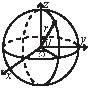
\includegraphics[width=25mm]{sphericalCoordinates.pdf}
\end{center}
\[\begin{array}{cc}
x = r\sin\theta\cos\phi & r = \sqrt{x^2+y^2+z^2}\\
y = r\sin\theta\sin\phi & \theta = \textrm{acos}(z/\sqrt{x^2+y^2+z^2})\\
z = r\cos\theta & \phi = \textrm{atan2}(y,x)
\end{array}\]

\subsection{Derivatives/Integrals}
\begin{align*}
	\dfrac{d}{dx}\arcsin x = \dfrac{1}{\sqrt{1-x^2}} &&& \dfrac{d}{dx}\arccos x = -\dfrac{1}{\sqrt{1-x^2}} \\
	\dfrac{d}{dx}\tan x = 1+\tan^2 x &&& \dfrac{d}{dx}\arctan x = \dfrac{1}{1+x^2} \\
	\int\tan ax = -\dfrac{\ln|\cos ax|}{a} &&& \int x\sin ax = \dfrac{\sin ax-ax \cos ax}{a^2} \\
	\int e^{-x^2} = \frac{\sqrt \pi}{2} \text{erf}(x) &&& \int xe^{ax}dx = \frac{e^{ax}}{a^2}(ax-1)
\end{align*}

Integration by parts:
\[\int_a^bf(x)g(x)dx = [F(x)g(x)]_a^b-\int_a^bF(x)g'(x)dx\]

\subsection{Sums}
\[ c^a + c^{a+1} + \dots + c^{b} = \frac{c^{b+1} - c^a}{c-1}, c \neq 1 \]
\begin{align*}
	1 + 2 + 3 + \dots + n &= \frac{n(n+1)}{2} \\
	1^2 + 2^2 + 3^2 + \dots + n^2 &= \frac{n(2n+1)(n+1)}{6} \\
	1^3 + 2^3 + 3^3 + \dots + n^3 &= \frac{n^2(n+1)^2}{4} \\
	1^4 + 2^4 + 3^4 + \dots + n^4 &= \frac{n(n+1)(2n+1)(3n^2 + 3n - 1)}{30} \\
\end{align*}

\subsection{Series}
$$e^x = 1+x+\frac{x^2}{2!}+\frac{x^3}{3!}+\dots,\,(-\infty<x<\infty)$$
$$\ln(1+x) = x-\frac{x^2}{2}+\frac{x^3}{3}-\frac{x^4}{4}+\dots,\,(-1<x\leq1)$$
$$\sqrt{1+x} = 1+\frac{x}{2}-\frac{x^2}{8}+\frac{2x^3}{32}-\frac{5x^4}{128}+\dots,\,(-1\leq x\leq1)$$
$$\sin x = x-\frac{x^3}{3!}+\frac{x^5}{5!}-\frac{x^7}{7!}+\dots,\,(-\infty<x<\infty)$$
$$\cos x = 1-\frac{x^2}{2!}+\frac{x^4}{4!}-\frac{x^6}{6!}+\dots,\,(-\infty<x<\infty)$$

\subsection{Probability theory}
Let $X$ be a discrete random variable with probability $p_X(x)$ of assuming the value $x$. It will then have an expected value (mean) $\mu=\mathbb{E}(X)=\sum_xxp_X(x)$ and variance $\sigma^2=V(X)=\mathbb{E}(X^2)-(\mathbb{E}(X))^2=\sum_x(x-\mathbb{E}(X))^2p_X(x)$ where $\sigma$ is the standard deviation. If $X$ is instead continuous it will have a probability density function $f_X(x)$ and the sums above will instead be integrals with $p_X(x)$ replaced by $f_X(x)$.

Expectation is linear:
\[\mathbb{E}(aX+bY) = a\mathbb{E}(X)+b\mathbb{E}(Y)\]
For independent $X$ and $Y$, \[V(aX+bY) = a^2V(X)+b^2V(Y).\]

\subsubsection{Discrete distributions}

\paragraph{Binomial distribution}
The number of successes in $n$ independent yes/no experiments, each which yields success with probability $p$ is $\textrm{Bin}(n,p),\,n=1,2,\dots,\, 0\leq p\leq1$.
\[p(k)=\binom{n}{k}p^k(1-p)^{n-k}\]
\[\mu = np,\,\sigma^2=np(1-p)\]
$\textrm{Bin}(n,p)$ is approximately $\textrm{Po}(np)$ for small $p$.

\paragraph{First success distribution}
The number of trials needed to get the first success in independent yes/no experiments, each wich yields success with probability $p$ is $\textrm{Fs}(p),\,0\leq p\leq1$.
\[p(k)=p(1-p)^{k-1},\,k=1,2,\dots\]
\[\mu = \frac1p,\,\sigma^2=\frac{1-p}{p^2}\]

\paragraph{Poisson distribution}
The number of events occurring in a fixed period of time $t$ if these events occur with a known average rate $\kappa$ and independently of the time since the last event is $\textrm{Po}(\lambda),\,\lambda=t\kappa$.
\[p(k)=e^{-\lambda}\frac{\lambda^k}{k!}, k=0,1,2,\dots\]
\[\mu=\lambda,\,\sigma^2=\lambda\]

\subsubsection{Continuous distributions}

\paragraph{Uniform distribution}
If the probability density function is constant between $a$ and $b$ and 0 elsewhere it is $\textrm{U}(a,b),\,a<b$.
\[f(x) = \left\{
\begin{array}{cl}
\frac{1}{b-a} & a<x<b\\
0 & \textrm{otherwise}
\end{array}\right.\]
\[\mu=\frac{a+b}{2},\,\sigma^2=\frac{(b-a)^2}{12}\]

\paragraph{Exponential distribution}
The time between events in a Poisson process is $\textrm{Exp}(\lambda),\,\lambda>0$.
\[f(x) = \left\{
\begin{array}{cl}
\lambda e^{-\lambda x} & x\geq0\\
0 & x<0
\end{array}\right.\]
\[\mu=\frac{1}{\lambda},\,\sigma^2=\frac{1}{\lambda^2}\]

\paragraph{Normal distribution}
Most real random values with mean $\mu$ and variance $\sigma^2$ are well described by $\mathcal{N}(\mu,\sigma^2),\,\sigma>0$.
\[ f(x) = \frac{1}{\sqrt{2\pi\sigma^2}}e^{-\frac{(x-\mu)^2}{2\sigma^2}} \]
If $X_1 \sim \mathcal{N}(\mu_1,\sigma_1^2)$ and $X_2 \sim \mathcal{N}(\mu_2,\sigma_2^2)$ then
\[ aX_1 + bX_2 + c \sim \mathcal{N}(\mu_1+\mu_2+c,a^2\sigma_1^2+b^2\sigma_2^2) \]

\subsection{Markov chains}
A \emph{Markov chain} is a discrete random process with the property that the next state depends only on the current state.
Let $X_1,X_2,\ldots$ be a sequence of random variables generated by the Markov process.
Then there is a transition matrix $\mathbf{P} = (p_{ij})$, with $p_{ij} = \Pr(X_n = i | X_{n-1} = j)$,
and $\mathbf{p}^{(n)} = \mathbf P^n \mathbf p^{(0)}$ is the probability distribution for $X_n$ (i.e., $p^{(n)}_i = \Pr(X_n = i)$),
where $\mathbf{p}^{(0)}$ is the initial distribution.

% \subsubsection{Stationary distribution}
$\mathbf{\pi}$ is a stationary distribution if $\mathbf{\pi} = \mathbf{\pi P}$.
If the Markov chain is \emph{irreducible} (it is possible to get to any state from any state),
then $\pi_i = \frac{1}{\mathbb{E}(T_i)}$ where $\mathbb{E}(T_i)$  is the expected time between two visits in state $i$.
$\pi_j/\pi_i$ is the expected number of visits in state $j$ between two visits in state $i$.

For a connected, undirected and non-bipartite graph, where the transition probability is uniform among all neighbors, $\pi_i$ is proportional to node $i$'s degree.

% \subsubsection{Ergodicity}
A Markov chain is \emph{ergodic} if the asymptotic distribution is independent of the initial distribution.
A finite Markov chain is ergodic iff it is irreducible and \emph{aperiodic} (i.e., the gcd of cycle lengths is 1).
$\lim_{k\rightarrow\infty}\mathbf{P}^k = \mathbf{1}\pi$.

% \subsubsection{Absorption}
A Markov chain is an A-chain if the states can be partitioned into two sets $\mathbf{A}$ and $\mathbf{G}$, such that all states in $\mathbf{A}$ are absorbing ($p_{ii}=1$), and all states in $\mathbf{G}$ leads to an absorbing state in $\mathbf{A}$.
The probability for absorption in state $i\in\mathbf{A}$, when the initial state is $j$, is $a_{ij} = p_{ij}+\sum_{k\in\mathbf{G}} a_{ik}p_{kj}$.
The expected time until absorption, when the initial state is $i$, is $t_i = 1+\sum_{k\in\mathbf{G}}p_{ki}t_k$.


\onecolumn

\makegrid

\end{document}
